\section{Introduction}

Titan is the only moon of the solar system with a thick hazy atmosphere which represents approximately 20\% of its apparent
diameter. This atmosphere is mainly composed of nitrogen and methane. The photo-dissociation of these molecules by the
UV light in the upper part of the atmosphere leads to the production of a large number of other hydrocarbons and nitriles as
trace species and to photochemical haze of aerosols. This haze is global and completely covers Titan. It controls
the thermal balance through its visible and thermal infrared properties \citep[e.g.][]{Bezard2018}.
It also veils the lower atmosphere and the surface that can be perceived in few methane windows in near infrared.

Although the haze was detected in the middle 70's, it was first imaged by Pioneer 11 \citep{Smith1980} and the two Voyagers
\citep{Smith1981, Smith1982, Sromovsky1981}. Titan's haze layer had several remarkable structures as a northern (winter)
polarhood, an interhemispheric asymmetry and a thin global detached haze layer (DHL) above the main global haze layer. It was
readily though that the detached haze layer had a dynamical origin \citep{Smith1981}. Photometric analysis allowed
to derive the extinction properties of both haze layers and evaluated the effective radius of the aerosols in the detached
haze ($\simeq 0.3 \mu$m) and in the main haze ($\simeq 0.4 \mu$m) layers \citep{Rages1983, Rages1983a}. Analysis show
that the detached haze layer appears due to a strong depletion in aerosols extinction around 300 km, yielding a distinct
layer above the main haze layer with a maximum extinction located around 350 km \citep{Rages1983}. Its horizontal extent was
very stable in pressure and it was reported at all the southern latitudes up to \ang{45}N where it connected to the northern
polar hood. The detached haze layer was re-observed twenty years after the Voyager flybys during Cassini first flyby in 2004
\citep{Porco2005}. The main change was in its altitude location at 500 km, which was 150 km higher than in 1981.
Again, it was a fairly homogeneous global shell above the main haze layer at a constant altitude with a
merging with the northern polarhood. Notably, while Voyager observations were performed after the northern spring equinox,
Cassini early observations occurred during the northern winter, that is half a season earlier (Fig.~\ref{fig:titan_seasons}).

\begin{figure}[!ht]
    \centering
    \includegraphics[width=\textwidth]{Fig/Titan_seasons.png}  % TODO: Update dates for Saturn and not Titan…
    \caption{Titan orbital position as function of the season, reported as solar longitude position ($L_s$).
             The Cassini mission covered almost half a Titan's year. Pioneer's and Voyagers' flybys are also reported
             as well as Huygens landing and ground based stellar occultations performed on Earth.}
    \label{fig:titan_seasons}
\end{figure}

The first attempt to explain the observation of the DHL is proposed by \cite{Toon1992}. They used a 1D microphysical
model where an \emph{ad hoc} vertical wind is added to maintain aloft the DHL particles at a constant altitude above the main
haze layer. Alternative scenarios were proposed to explain the DHL from pure microphysical processes. \cite{Chassefiere1995}
investigated the case of two different aerosol production layers. They proposed that the uppermost layer (500-1000 km)
produces fluffy aggregates that could be swept horizontally by winds, generating a detached haze layer. They also
propose an alternative scenario where aerosols settle downward and interact with macromolecules from the main haze layer,
produced by the lower production zone (around 350-400 km). In the latter case, the interaction would produce by some
way an optical gap. However, they clearly favorized the scenario involving winds which would match all the constraints
known at that time. In the same vein, \cite{Lavvas2009} proposed a scenario based on a pure microphysical process. Aerosols
are produced at high altitude, as in \cite{Chassefiere1995} hypothesis, growing as spheres down to levels around 500 km.
But there, the detached haze is produced by a sudden change in the fractal dimension of the aerosols. This produces a
sharpe change in the microphysical properties, and an artificial optical gap. However, it is unclear how this model for the
production of the detached haze layer would be augmented to account for the seasonal evolution of the altitude,
disappearance, and reappearance (as described below).

Later, with a 2D-General Climate Model (GCM) accounting for the transport of haze by dynamics and the radiative
feedback it was possible to reproduce and explain the mechanism that produces the DHL \citep{Rannou2002}. It was also
demonstrated that this feedback strongly enhances the wind speed due to the thick polar haze cap at winter pole built
by the circulation. In return, this cap enhances the cooling to space during the polar night \citep{Rannou2004} an
reinforce the circulation. Due to Titan's obliquity (\ang{27}) and the slow rotation rate, seasons are well
marked and circulation cells span over all the planet. This situation leads to the formation of a
broad ascending circulation in the summer hemisphere able to lift aerosols up to high altitudes where they remain
suspended and are transported through mid-latitudes to the winter polar region where they are transported by
subsidence (Fig.~\ref{fig:titan_atm_circulation}). In this scenario, the location of the DHL corresponds to the area
where the settling speed is compensated by upward wind and evolves with the changes of illumination along the seasons.
More sophisticated 3D-GCM improved the understanding of the haze cycle, including the formation of the detached haze,
and basically confirmed this picture \citep{Lebonnois2012,Larson2015}. This formation mechanism implies that the DHL
is a blending of aerosols newly produced and falling from above and older and larger aerosols produced in the
stratosphere and lifted by circulation.
Although the GCM's results differ in some aspects with observations, they are able to capture the main picture behind
the existence of the DHL.

\begin{figure}[!ht]
    \centering
    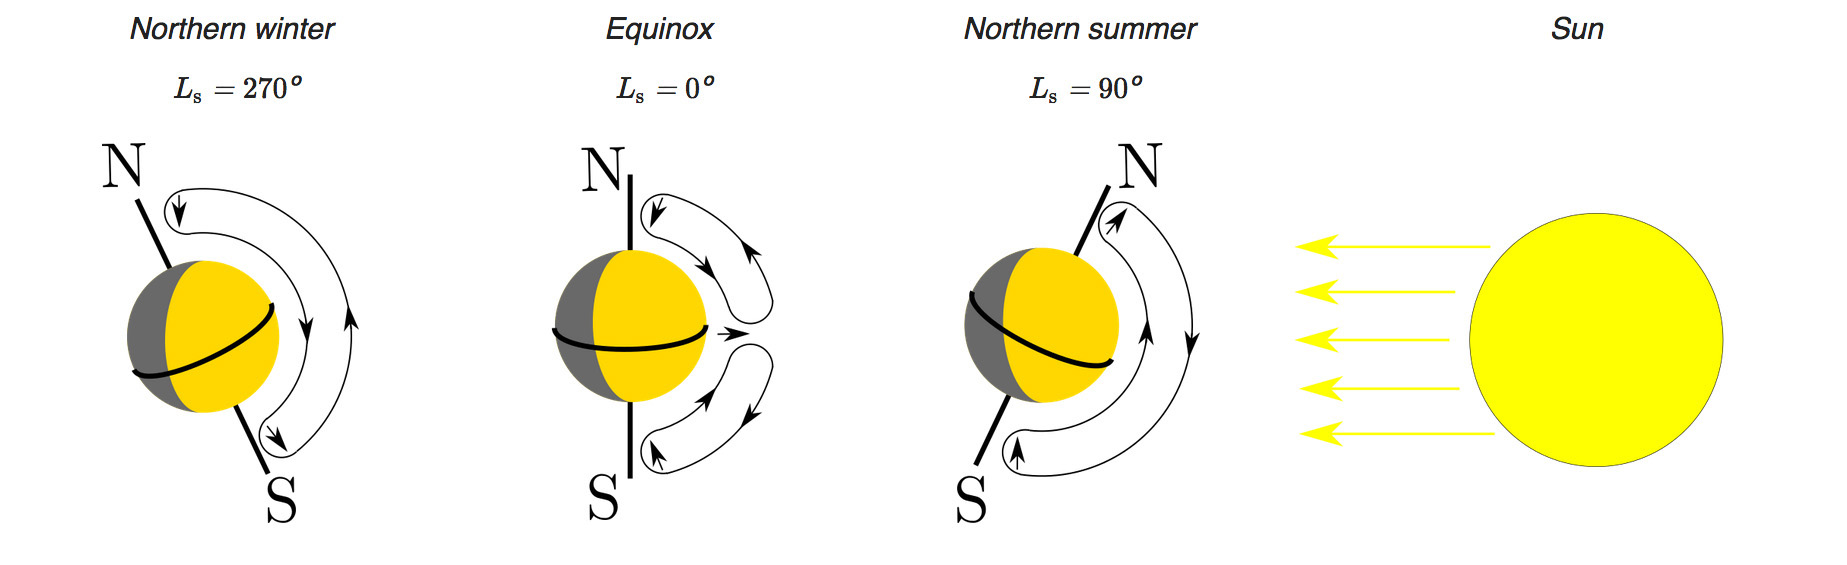
\includegraphics[width=\textwidth]{Fig/Atmsopheric_circulation.jpg}  % TODO: Add vectorized image
    \caption{Synthetic representation of Titan atmospheric circulation as a function of the season.}
    \label{fig:titan_atm_circulation}
\end{figure}

Photometric studies performed with Cassini data taken before the equinox in 2009 provide complementary observations
of the DHL \citep{Cours2011, Koskinen2011, Seignovert2017}.
On one hand, the authors used the light intensity scattered at the limb in UV (338 nm)
at different phase angles measured by ISS. On the other hand, a single value of the tangential opacity in VUV (187 nm)
was retrieved from UVIS observations during stellar occultations.
The results show the presence of large aerosols in the DHL with an effective bulk radius $\simeq 0.2\ \mu$m,
producing all the UV scattering, while small nanometric aerosols are needed to explain most of the VUV
extinction \citep{Cours2011}, which is quite consistent with a DHL made of two different populations of
aerosols.

\cite{West2011} also reported a rapid collapse of the detached haze layer starting just before the equinox. The altitude of
the DHL descended by about 80 km in 200 terrestrial days and by 30 km more in about 300 terrestrial days. A simple
extrapolation of the altitude of the DHL with time indicated that it would be at the same altitude as observed by Voyager
exactly one Titan year after the Voyager epoch. \cite{West2011} concluded that such a result was coherent with a seasonal
cycle of the DHL.  They compared their results with a 2D-GCM \citep{Rannou2002} and made a prediction about the reappearance of the
DHL several years later (2013-2016) at its initial altitude (around 500 km). \cite{Lebonnois2012} and \cite{Larson2015} made
similar predictions but with a reappearance of the DHL a bit later, around the next northern summer solstice ($L_S=\ang{95}$
and $\ang{70}-\ang{80}$, respectively). In practice, \cite{West2018} found that the DHL reappeared in early 2016
($L_S=\ang{73}-\ang{76}$) at 480 km, several months before the solstice (mid-2017). They followed the cycle of the DHL at the equator
and retrieved the haze extinction profile in the CL1-UV3 filter combination.
Its reappearance was much more complex than predicted. This early 2016 detached haze layer
dropped in altitude down to 470 km within a terrestrial year and vanished while a new DHL emerged again around 500 km. This
new layer appeared quite stable until the end of the Cassini mission (september 2017, $L_S=\ang{91}$). Unfortunately, no other
mean exists to further probe the DHL and nothing is known about the fate of the detached haze after this date.
% TODO: Add ground base stellar occultations ?

\medskip

In the present work, we perform a systematic latitude-altitude mapping of the detached haze layer between 350 to 600 km.
This covers the period between July 2004 (half a season after the northern winter solstice) and the end of
the mission in September 2017 (after the summer solstice).
We used all the UV3 observations acquired by the Narrow Angle Camera (NAC) of ISS camera onboard Cassini.
We used exactly the same model as \cite{West2018}, that is a ray tracing model in spherical shell for the single scattering albedo
and a correction for the multiples scattering.

The outline of the article is as follow. In the next section (\textbf{section 2}), we first give a global presentation of
the available dataset and the criterion we use to select the images used in our study.
Then we describe the main principle of the retrieval model that is used for the analysis and the retrieval method.
In \textbf{section 3} we present the results of the photometric analysis as latitude -
altitude panels showing the spatial distribution of the DHL and the upper part of the main haze layer.
The seasonal cycle of the DHL is split in four specific periods between 2004 and 2017.
This section has then 4 subsections for each periods where we explain in detail the main characteristics of the haze and
its evolution.
\textbf{Section 4} is dedicated to the study of specific sets of observations that allow to probe short time,
short term or diurnal variations. We first describe how the data were selected and then what they reveal about Titan atmosphere.
In the \textbf{section 5}, we make comparisons between our results and results obtained at the same location and the same time with UVIS.
We also make comparisons between our results and prediction made by two Titan 3D-GCM about the detached haze layer and its evolution.
The conclusion and the perspective of this work are given in \textbf{section 6}.
